% !TEX program = xelatex
% =============================================================================
%  ICCIES 2027 submission (Springer CCIS / LNCS style)
%
%  Build with XeLaTeX only:
%      latexmk -xelatex main.tex     (or xelatex + bibtex + xelatex + xelatex)
%  latexmk picks the engine up from latexmkrc, so a bare `latexmk main.tex`
%  also works.
%
%  The Vietnamese examples carry tone-marked letters (lủ, nhục, sủa, mẹ) from
%  Unicode's Latin Extended Additional block, which T1/pdflatex cannot typeset:
%  it reports "Unicode character ... not set up for use with LaTeX" and drops
%  the letter, and the resulting Computer Modern setting needs 17 pages instead
%  of the 15 allowed.
% =============================================================================
\documentclass[runningheads]{llncs}

\usepackage{iftex}
\ifPDFTeX
  % Refuse to build: under pdfLaTeX the Vietnamese examples lose their tone
  % marks (T1 has no such glyphs) and the Computer Modern default needs 17 pages
  % instead of the 15 allowed.  \stop is required because Overleaf and editors
  % run TeX in nonstopmode, where \PackageError alone only prints the message and
  % then carries on producing a silently wrong PDF.
  \PackageError{iccies2027}{\%
    Build this paper with XeLaTeX, not pdfLaTeX.\MessageBreak
    On Overleaf: Menu -> Compiler -> XeLaTeX.\MessageBreak
    Locally: latexmk -xelatex main.tex}{\%
    Vietnamese tone marks do not exist in T1, so pdfLaTeX reports\MessageBreak
    "Unicode character ... not set up for use with LaTeX" for every example,\MessageBreak
    drops the letters, and needs 17 pages instead of the 15 allowed.}\%
  \stop
\else
  \usepackage{fontspec}
  % CMU Serif (Computer Modern Unicode): Latin Modern look with full
  % Vietnamese glyph support (roman + italic + small caps).
  % Installed via MiKTeX cm-unicode package.
  \setmainfont{CMU Serif}
\fi

\usepackage{graphicx}
\usepackage{booktabs}
\usepackage{array}
\usepackage{tabularx}
\usepackage{amsmath}
\usepackage{amssymb}
\usepackage{url}
\usepackage[hidelinks]{hyperref}
\usepackage{orcidlink}
% The llncs class asks authors not to change the printing area or the caption
% spacing (llncsdoc, Sect. 2.1).  Only the float-placement policy and the
% separations around floats are relaxed here, so that five floats share the
% pages with the text inside the 15-page ICCIES limit; text geometry, heading
% and caption spacing keep the class defaults.
\renewcommand{\topfraction}{1.0}
\renewcommand{\bottomfraction}{1.0}
\renewcommand{\textfraction}{0.05}
\renewcommand{\floatpagefraction}{0.9}
\setcounter{totalnumber}{6}
\setlength{\textfloatsep}{8pt plus 2pt minus 2pt}
\setlength{\floatsep}{8pt plus 2pt minus 2pt}
\setlength{\intextsep}{0pt plus 1pt minus 1pt}
\setlength{\emergencystretch}{3em}

\newcommand{\model}[1]{\textsc{#1}}
\newcommand{\hate}{\textsc{hate}}
\newcommand{\off}{\textsc{offensive}}
\newcommand{\clean}{\textsc{clean}}

\linespread{0.98}\selectfont
\begin{document}

\title{An Explainable Hybrid of Lexicon Rules and Multilingual
  Transformers for Vietnamese Sensitive Speech Detection}
\titlerunning{An Explainable Hybrid for Vietnamese Sensitive Speech Detection}

% ORCID iDs are optional in the class but expected by Springer for the
% corresponding authors: replace the commented placeholders below with the real
% iDs (https://orcid.org) before submitting to CMT.
\author{
  Pham Kha Vy\inst{1}\,\orcidlink{0009-0008-1958-3070}
  \and
  Cao Hong Nga\inst{1}\textsuperscript{(*)}\,\orcidlink{0000-0003-0343-6523}
  \and
  Jia-Ching Wang\inst{2}\textsuperscript{(*)}\,\orcidlink{0000-0003-0024-6732}
}

\authorrunning{K. V. Pham,  H. N. Cao, and J. C. Wang}
\institute{
  FPT University, Can Tho, Vietnam,
  \email{phamkhavycm2004@gmail.com},
  \email{caohongnga@gmail.com}\\
  \and
  Department of Computer Science \& Information Engineering, National Central University, Taoyuan, Taiwan,  \email{jcw@csie.ncu.edu.tw}\\
  \textsuperscript{(*)}are the corresponding authors.
}

\maketitle

\begin{abstract}
  Hate speech detection is an essential component of content moderation on social media, where harmful comments spread rapidly and platforms are required to provide clear justifications for content removal decisions. Detecting hate and offensive speech in Vietnamese presents several challenges due to the limited availability of linguistic resources and the widespread use of obfuscation techniques, such as teencode, diacritic omission, character separation, and profanity abbreviation. Furthermore, the distinction between "hate" and "insult" depends not only on the vocabulary used but also on the intensity of the expression and the target of the attack. To address these challenges, this study proposes a hybrid framework for Vietnamese sensitive content detection that integrates a rule-based detection mechanism with a Transformer-based deep learning model, namely mDeBERTa-v3. The proposed framework aims to identify both hate speech and offensive language by leveraging the complementary strengths of lexical rules and contextual representations. Experiments conducted on the ViHSD dataset achieved a macro-F1 score of 66.02\% on the test set, representing a modest improvement over the mDeBERTa-v3 baseline, which obtained 65.75\%. Although the improvement is relatively small, the results suggest that incorporating rule-based detection can provide additional benefits beyond the standalone Transformer model. Nevertheless, the rule-based component requires further refinement, particularly in terms of lexical coverage and quality, to enhance its contribution to the overall framework.
  \keywords{Sensitive content detection \and Rule-based sensitive detection \and Transformer-based sensitive detection \and
    Hybrid system \and Lexicon rules.}
\end{abstract}
\section{Introduction}
\label{sec:intro}

Vietnam has one of Southeast Asia's fastest-growing social-media user bases, and the
volume of Vietnamese text its platforms must moderate keeps rising. The language is low-resource
and its social-media register is hard: writers abbreviate profanity into
\emph{teencode} (\texttt{dm}, \texttt{cc}, \texttt{vl}), drop diacritics, stretch
letters, insert separators, and rely on irony or quotation to be hostile without
writing a dictionary slur.

The release of UIT-ViHSD \cite{luu2021vihsd}, roughly 33k comments labelled
\clean{}, \off{} or \hate{}, made supervised transformer fine-tuning the default.
PhoBERT \cite{nguyen2020phobert}, ViSoBERT \cite{nguyen2023visobert}, multilingual
DeBERTa-v3 variants \cite{he2021deberta,he2023debertav3,liu2024mdeberta} and
ViHateT5 \cite{nguyen2024vihatet5} all perform well, yet on UIT-ViHSD strong encoders
plateau: about 83\% of test comments are \clean{}, \hate{} and \off{} overlap in
annotation, and their boundary is often intensity rather than lexical content.

Two problems follow. First, \emph{opacity}: removals need inspectable reasons, yet
post-hoc attribution (LIME \cite{ribeiro2016why}, SHAP \cite{lundberg2017shap})
approximates the model. Second, \emph{brittleness on surface form}: a transformer may
never see obfuscated profanity (\texttt{d.m}, \texttt{đ*m}), while a lexicon matches
such variants explicitly.

We ask: \emph{can a lexicon be attached to a transformer as an evidence channel, so
decisions where the rule fires carry inspectable lexical support, without degrading accuracy?} We
do not claim higher accuracy; we claim the small change is \emph{attributable}: each
changed decision traces to a specific mechanism, exposing a systematic failure that
aggregate metrics hide.

We fuse a 668-term Vietnamese hate-speech lexicon with four mDeBERTa-v3 backbones
differing only in head and optimisation recipe. The rule engine normalises the comment, builds
accent-less, leet, repeat-collapsed and separator-stripped views, scores each matched
span by severity, confidence, match type and context, and aggregates per label; fusion
mixes channels and applies frozen per-channel thresholds.

Contributions: (i) a frozen, reproducible hybrid protocol with an independent,
inspectable rule channel; (ii) per-decision provenance assigning every change to a
rule- or threshold-driven mechanism; (iii) a behavioural audit of the rule channel
with a cue taxonomy; (iv) an analysis of missed corrections motivating
evidence-gated fusion; (v) case studies with matched spans and scores.
\section{Related Work}
\label{sec:related}

\paragraph{Lexicon-based detection.}
Pre-transformer detectors used lexicons and hand-written surface features
\cite{waseem2016hateful}: Gitari et al.\ \cite{gitari2015lexicon} score a comment from a
curated profanity lexicon and apply rules over matched phrases---inspectable, but
hand-curated, with recall bounded by the list. Wiegand et al.\
\cite{wiegand2018inducing} automate that induction step, the closest antecedent to our
entry severity and confidence. Schmidt and Wiegand \cite{schmidt2017survey} explain the
move to learned models: the \hate{}/\off{} boundary is combinatorial, not lexical.
Davidson et al.\ \cite{davidson2017automated} found the two classes share most surface
vocabulary---which makes our channel over-fire on \off{}---and surveys
\cite{fortuna2018survey} list the recurring difficulties: imbalance, subjectivity,
overlap, obfuscation, domain shift. We treat these as the object of analysis, not
obstacles to a classifier.

\paragraph{Vietnamese resources and models.}
ViHSD \cite{luu2021vihsd} is the reference three-way benchmark, ViCTSD
\cite{nguyen2021victsd} provides related data, and ViCM \cite{nguyen2026vicm} adds
code-mixed comments. PhoBERT \cite{nguyen2020phobert} adapts RoBERTa to Vietnamese,
ViSoBERT \cite{nguyen2023visobert} is pre-trained on social media, and ViHateT5
\cite{nguyen2024vihatet5} casts the task as generation. ViHOS \cite{hoang2023vihos}
annotates the \emph{spans} that make a comment hateful, the closest Vietnamese work to
our notion of evidence; our spans come from a lexicon matcher, but the motivation is
the same. SMTCE \cite{nguyen2022smtce} standardises evaluation, hence our macro-F1
focus.

\paragraph{Multilingual transformers.}
mBERT \cite{devlin2019bert} and XLM-R \cite{conneau2020xlmr} established multilingual
pre-training; DeBERTa \cite{he2021deberta} introduced disentangled attention, and
DeBERTa-v3 \cite{he2023debertav3} adds ELECTRA-style pre-training, whose
\texttt{microsoft/\allowbreak mdeberta-v3-base} checkpoint \cite{liu2024mdeberta} we
fine-tune.

\paragraph{Explainability and hybrid systems.}
HateXplain \cite{mathew2021hatexplain} made human rationales and explanation quality
benchmark quantities. LIME \cite{ribeiro2016why} and SHAP \cite{lundberg2017shap} are
model-agnostic but do not guarantee that highlighted tokens are the ones the decision
used. Our rule channel is part of the decision function, so its matched spans are
\emph{faithful by construction} for the lexical component, though the neural component
remains opaque. We settle the accuracy question with a paired test, analyse provenance,
and report the rule channel's own error profile and the direction of every
rule-induced change; to our knowledge, this audit is new for Vietnamese hate speech.

\section{Data and Lexicon}

\label{sec:data}

\subsection{The UIT-ViHSD corpus}

\label{sec:vihsd}

We use UIT-ViHSD \cite{luu2021vihsd}, Vietnamese social-media comments annotated
with three mutually exclusive labels: \clean{} (no offensive content), \off{}
(offensive language not targeting a protected group as hate speech) and \hate{}
(hateful or seriously derogatory). The \off{}/\hate{} distinction depends on target
and intensity rather than on a particular word, so a lexical rule engine is
insufficient on its own.

After cleaning, the corpus has 33{,}398 comments; every system reads the same fixed
split, whose SHA-256 digest is stored and re-checked per run. Training: 24{,}046
(2{,}556 \hate{}, 1{,}605 \off{}, 19{,}885 \clean{}); validation 2{,}672
(270/212/2{,}190); test 6{,}680 (688/444/5{,}548).

The test split is imbalanced: 83.05\% \clean{}, 10.30\% \hate{} and 6.65\% \off{},
so accuracy is a poor headline metric---a constant \clean{} predictor already reaches
0.8305---and macro-F1 is primary, always with per-class F1. The 6{,}680 test rows
contain 6{,}571 distinct texts (109 duplicated rows), kept because removing them would
change the frozen test set; one appears twice among the 15 regressions, which thus
cover 14 distinct texts.

\subsection{The hate-speech lexicon}

\label{sec:lexicon}

The rule engine is driven by a Vietnamese hate-speech lexicon of \textbf{668 entries},
mined and labelled from the \emph{training} portions of UIT-ViHSD; R-UIT-ViHSD
\cite{bontoriTdtu}; and ViCM \cite{nguyen2026vicm}. The three training splits yield
1{,}062 candidate terms (first attested 257/665/140 in UIT-ViHSD/ViCM/R-UIT-ViHSD); manual labelling and
filtering reduce these candidates to the 668 entries below. No evaluation split is sampled; each entry records
its supporting corpora (414 of 668 occur in all three).

An exact-text cross-corpus audit found 895 of 6{,}680 UIT-ViHSD test rows (13.4\%)
with a matching text in auxiliary corpus material used for lexicon development---620
distinct test texts also in the Bontori/R-UIT-ViHSD training partition---a potential
source of lexicon-construction leakage. To assess its effect, we rebuilt the lexicon
excluding those texts (671 entries vs. 668 canonical). Main results use the canonical
lexicon; leak-free results are in Sect.~\ref{sec:leak-free-sensitivity}.

Each entry stores the surface term and canonical form, a label (\hate{} or \off{}) with
per-label severity, a training-estimated confidence, a context-required flag, and a
review status (\emph{verified} or \emph{auto}), retained in the evidence record.

The lexicon is deliberately not a list of slurs: 551 of 668 (82.5\%) are multi-word
constructions (\emph{mẹ cha}, \emph{con mẹ}, \emph{ngu hơn}) and 524 (78.4\%) are
context-required, since Vietnamese insults work by comparison and implication rather
than a single taboo word. Only 74 entries are \off{} against 594 \hate{}, so the engine
is weak on \off{} and fusion keeps that channel mostly neural. The lexicon is
\emph{editable}, \emph{deterministic} and \emph{inspectable} (each score decomposes
into term, match type and context factor).

\paragraph{Ethics of examples.}
All quoted comments are public UIT-ViHSD test comments. Because they contain profanity
and slurs, we mask offending characters with \texttt{*} in every table; evaluation
runs on unmasked text. No user identifiers are reproduced, and names inside comments
are part of the public corpus text.
\section{Method}
\label{sec:method}

\begin{figure}[ht]
\centering
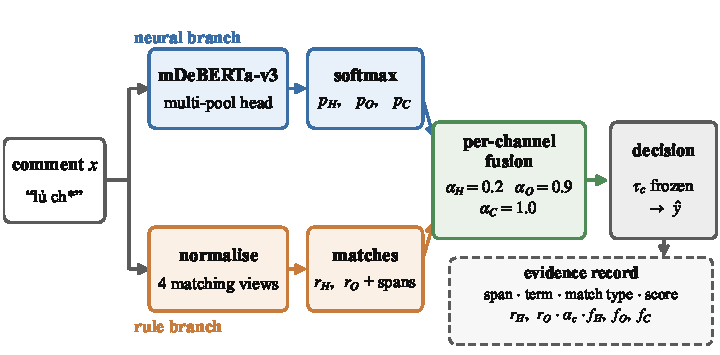
\includegraphics[width=0.80\textwidth]{figures/architecture.pdf}
\caption{The hybrid. A comment enters two branches: the neural branch produces class
probabilities, the rule branch per-label lexical scores and the spans that produced
them. Fusion mixes each channel with its own weight $\alpha_c$, and frozen per-channel
thresholds turn the three scores into a label; the evidence record is emitted with the
decision. Weights and thresholds shown were selected on validation for the focused
backbone.}
\label{fig:architecture}
\end{figure}

The hybrid has three parts: a rule engine that produces lexical scores and spans, a
transformer that produces class probabilities, and a fusion layer that combines them
channel by channel (Fig.~\ref{fig:architecture}). The branches share no parameters,
which allows the rule branch to be audited on its own.

\subsection{The lexical rule engine}
\label{sec:rule-engine}

\paragraph{Normalisation and views.}
The comment is Unicode-normalised to NFC, invisible characters removed, whitespace
collapsed, runs shortened to at most three, lower-cased while keeping diacritics. An
offset map reports a cleaned-view match as an original span. Auxiliary views handle
accent-less, leet, repeat-collapsed and separator-stripped (\texttt{n g u}) text.
Each hit records term, label, view, raw span and match type (e.g.\ \emph{exact},
\emph{accentless\_alias}, \emph{leet}, \emph{separator\_inserted}, \emph{fuzzy}).

\paragraph{Scoring.}
Every match $i$ receives
\begin{equation}
s_i \;=\; \sigma_{\ell(i)} \cdot c_i \cdot m_i \cdot \kappa_i ,
\label{eq:match}
\end{equation}
where $\sigma_{\ell(i)}$ is the severity of the matched label ($0.95$ for
\hate{}, $0.60$ for \off{} after tuning), $c_i$ the entry confidence from the
training split, $m_i$ the match-type factor and $\kappa_i$ a context factor for
quotation, negation and context-required terms. Matches of one label are
de-duplicated and aggregated with a saturating sum over at most $K=10$ matches:
\begin{equation}
r_\ell \;=\; 1-\prod_{i\in T_\ell}\left(1-s_i\right).
\label{eq:aggregate}
\end{equation}
For fusion they become a three-channel pseudo-probability
\begin{equation}
\tilde{\mathbf r} \;=\; \frac{1}{1+\min(r_H,r_O)}
\begin{bmatrix} r_H \\ r_O \\ 1-\max(r_H,r_O) \end{bmatrix},
\label{eq:pseudo}
\end{equation}
which preserves the ordering of the two toxic channels while placing \clean{} on
the same scale. When the rule is silent, $\tilde{\mathbf r}=(0,0,1)$: no evidence
is treated as maximal cleanliness evidence, an assumption
Sect.~\ref{sec:analysis} tests.

\paragraph{Tuning.}
Scoring weights are tuned on validation by greedy coordinate descent, thresholds
re-optimised per candidate; the test set is never loaded. The search made the engine more
aggressive (severity \hate{} $0.95$, accentless-alias $0.0$, repeat-collapsed $0.4$,
combined-obfuscation $0.3$, negation and context-required $1.0$): validation preferred
more matches over cautious ones.

\subsection{The neural branch}
\label{sec:neural}

We fine-tune \texttt{microsoft/mdeberta-v3-base}
\cite{he2023debertav3,liu2024mdeberta}. The focused backbone
(\model{sensitiveai-vi-custom}) uses a multi-pool head: \texttt{[CLS]}, mean and max
pooling concatenated, projected to a 512-dim bottleneck (dropout $0.1$), then three
logits. Training: cross-entropy, AdamW \cite{loshchilov2019adamw}, linear schedule
with 10\% warm-up, lr $3\times10^{-5}$, batch 16, max length 256, up to 30 epochs,
early stopping on validation macro-F1. Three further backbones share the encoder with
different recipes: standard head; two-stage with discriminative learning rates and
focal loss \cite{lin2017focal}; three-stage curriculum \cite{bengio2009curriculum}
with manual class weights.

\subsection{Fusion and decision}
\label{sec:fusion}

Let $p_c$ be the transformer probability for class $c$ and $\tilde r_c$ the
renormalised rule score. Per-channel fusion is
\begin{equation}
f_c \;=\; \alpha_c\,p_c \;+\; (1-\alpha_c)\,\tilde r_c,
\qquad c\in\{\hate{},\off{},\clean{}\}.
\label{eq:fusion}
\end{equation}
A single global $\alpha$ is the special case $\alpha_H=\alpha_O=\alpha_C$. A class
is \emph{accepted} when $f_c\ge\tau_c$; the accepted class with the highest $f_c$
wins, and if none is accepted the decision falls back to $\arg\max_c f_c$.

We compare four families: global $\alpha$ with argmax, global $\alpha$ with
thresholds, a multinomial logistic meta-classifier over six scores, and per-channel
$\alpha$ with thresholds, all selected on validation. The per-channel variant is primary:
classes have different rule behaviour (precise on \hate{}, weak on \off{}, uninformative
on \clean{}). Validation finds $\alpha_H=0.2$, $\alpha_O=0.9$, $\alpha_C=1.0$ and
$\tau_H=0.14$, $\tau_O=0.66$, $\tau_C=0.60$.

\subsection{Evidence record and protocol}
\label{sec:evidence}

For every comment the system emits, with the label, an evidence record: matched
raw-text spans, each span's term and label, matching view and match type, per-match
score, aggregated rule scores, per-channel weights and the three fused scores. Given
the record and the transformer probabilities, a reviewer can recompute the decision
exactly---our meaning of \emph{faithful by construction} for the lexical channel, while
the neural contribution remains a black box.

\section{Experimental Setup}
\label{sec:setup}

\subsection{Backbones and tuning}
\label{sec:backbones}

Four backbones are evaluated, all using \texttt{microsoft/mdeberta-v3-base} with the
same tokenizer, split and evaluation code and differing only in head and optimisation
recipe. The focused model, \model{sensitiveai-vi-custom}, gives the clearest positive
net effect (23 corrections, 15 regressions) and is thus the clearest subject for
studying what fusion changes.

Rule-engine weights are tuned by greedy coordinate descent over the scoring
parameters, with the three decision thresholds re-optimised on validation macro-F1
over a 101-point grid at every candidate; the search never touches the lexicon. Fusion
uses the same discipline: thresholds by coordinate descent over the same grid for three
rounds, per-channel weights by coordinate ascent from the AI-only corner, and a
multinomial logistic meta-classifier on the six validation features.

\subsection{Metrics and implementation}
\label{sec:metrics}

Macro-F1 is primary (Sect.~\ref{sec:vihsd}). We report accuracy and per-class
precision, recall and F1, and evaluate differences with two paired tests: a paired
bootstrap over comments (10{,}000 resamples) for the macro-F1 difference
\cite{efron1993bootstrap}, and an exact McNemar test on the correctness contingency
table \cite{mcnemar1947note}, asking whether the aggregate moved and whether the
pattern of individual decisions changed, respectively.

The transformer uses PyTorch and Hugging Face Transformers
\cite{wolf2020transformers}; metrics follow the scikit-learn definitions and are
computed by one shared evaluator. The rule engine is pure
Python, runs on CPU, and processes a comment in 0.20\,ms on average (median 0.15\,ms),
roughly 4{,}900 comments per second, so it can run on every comment rather than as
a sampled audit.

\subsection{Reproducibility}
\label{sec:repro}

The split is hashed and re-checked, and the analysis script asserts that the rule
scores shipped with the fusion predictions match the frozen tuned output---an earlier
version read the \emph{untuned} scores and over-reported rule coverage threefold.

\section{Results}

\label{sec:results}

\subsection{Model-selection context}

We retain \texttt{sensitiveai-vi-custom} as a focused, exploratory case study for
tracing decision provenance---a post-hoc analysis, not a confirmatory validation-based
selection. The strongest standalone backbone by validation macro-F1 is
\texttt{sensitiveai-vi-customdlr2stage} (70.89\%), also strongest on test (66.38\%), so
the fusion results are not evidence that the focused backbone is best standalone.

\subsection{The hybrid does not improve accuracy}

\label{sec:no-accuracy-gain}

Table~\ref{tab:fusion-variants} reports every variant. AI alone reaches 65.75\%
macro-F1 and 87.62\% accuracy; the per-channel hybrid reaches 66.02\% and 87.74\%, a gain
of 0.27\% and eight more correct comments (5{,}861 vs. 5{,}853), concentrated in
\hate{}: F1 rises 58.30\% to 59.06\% via recall (53.34\% to 54.94\%) at a small precision
cost (64.27\% to 63.85\%), while \off{} and \clean{} barely move.

Per-channel weights add 0.10\% over a global weight (65.83\% to 65.93\%), thresholds
a further 0.09\%. The logistic meta-classifier is worse than AI alone (65.13\%): six
features on 2{,}672 validation comments overfit. Thresholds make the rule engine
usable alone (52.58\% vs.\ 47.14\% with argmax).

\begin{table}[ht]
\centering
\scriptsize
\setlength{\tabcolsep}{3pt}
\caption{Decision-level variants for the focused backbone
(\model{sensitiveai-vi-custom}) on test. Every variant reads the same frozen
scores; only mixing and the decision rule differ; the last row is primary.
\emph{Per-class columns are F1 (in percent)}; best macro-F1 in bold. Rule-only rows are scored
inside the fusion pipeline on renormalised rule scores; the standalone engine with
its own thresholds is reported in the text.}
\label{tab:fusion-variants}
\begin{tabular}{lccccc}
\toprule
System & Acc. & Macro-F1 & \hate & \off & \clean \\
\midrule
AI only (argmax)                      & 87.62 & 65.75 & 58.30 & 44.93 & 94.03 \\
Rule only (argmax)                    & 84.94 & 47.14 & 48.67 & 0.00 & 92.74 \\
Rule only (frozen thresholds)         & 84.21 & 52.58 & 41.02 & 23.89 & 92.84 \\
\midrule
Fusion, global $\alpha$ (argmax)      & 87.69 & 65.83 & 58.51 & 44.90 & 94.08 \\
Fusion, global $\alpha$ (thresholds)  & 87.69 & 65.83 & 58.51 & 44.90 & 94.08 \\
Fusion, logistic meta-classifier      & 86.26 & 65.13 & 58.18 & 43.79 & 93.41 \\
Fusion, per-channel $\alpha$ (argmax) & 87.74 & 65.93 & 58.82 & 44.88 & 94.08 \\
Fusion, per-channel (thresholds)      & 87.74 & \textbf{66.02} & 59.06 & 44.94 & 94.07 \\
\bottomrule
\end{tabular}
\end{table}


Table~\ref{tab:precision-recall} gives precision and recall, overall (macro) and
per label. The hybrid's \hate{} gain is recall-driven (53.34\% to 54.94\%) at a small
precision cost (64.27\% to 63.85\%); macro precision rises 68.43\% to 68.74\% and macro
recall 63.59\% to 63.83\%.

\vspace{12pt}
\begin{table}[ht]
\centering
\scriptsize
\setlength{\tabcolsep}{2pt}
\caption{Precision and recall on test for the focused backbone
(\model{sensitiveai-vi-custom}), over the same eight systems as
Table~\ref{tab:fusion-variants}. Per-class columns are precision (P)
and recall (R) in percent; macro averages are unweighted means. Best value in
each column is bold. Different systems win different columns: the
logistic meta-classifier has the highest recall but the lowest
macro-F1 (Table~\ref{tab:fusion-variants}), which aggregate F1 hides.}
\label{tab:precision-recall}
\begin{tabular}{lcccccccc}
\toprule
System & \multicolumn{2}{c}{\hate} & \multicolumn{2}{c}{\off} & \multicolumn{2}{c}{\clean} & \multicolumn{2}{c}{Macro} \\
\cmidrule(lr){2-3}\cmidrule(lr){4-5}\cmidrule(lr){6-7}\cmidrule(lr){8-9}
 & P & R & P & R & P & R & P & R \\
\midrule
AI only (argmax) & 64.27 & 53.34 & 48.44 & 41.89 & 92.58 & 95.53 & 68.43/63.59 \\
Rule only (argmax) & 46.90 & 50.58 & 0.00 & 0.00 & 89.69 & \textbf{96.00} & 45.53/48.86 \\
Rule only (thresholds) & 62.50 & 30.52 & 23.48 & 24.32 & 90.19 & 95.66 & 58.72/50.17 \\
Fusion, global $\alpha$ (argmax) & 64.56 & 53.49 & 48.68 & 41.67 & 92.58 & 95.62 & 68.61/63.59 \\
Fusion, global $\alpha$ (thresholds) & 64.56 & 53.49 & 48.68 & 41.67 & 92.58 & 95.62 & 68.61/63.59 \\
Fusion, logistic meta-classifier & 53.47 & \textbf{63.81} & 45.61 & \textbf{42.12} & \textbf{94.26} & 92.57 & 64.45/\textbf{66.17} \\
Fusion, per-channel $\alpha$ (argmax) & \textbf{64.91} & 53.78 & 48.94 & 41.44 & 92.55 & 95.66 & \textbf{68.80}/63.63 \\
Fusion, per-channel (thresholds) & 63.85 & 54.94 & \textbf{49.73} & 40.99 & 92.64 & 95.55 & 68.74/63.83 \\
\bottomrule
\end{tabular}
\end{table}


\vspace{6pt}
\begin{figure}[ht]
\centering
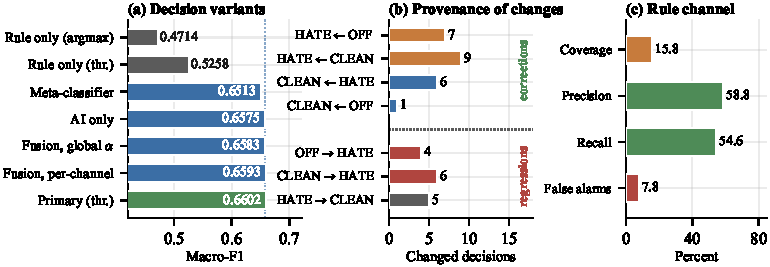
\includegraphics[width=0.85\textwidth]{figures/results.pdf}
\caption{Focused backbone. (a)\ Macro-F1 of each variant (dotted: AI-only).
(b)\ Provenance of the 38 changed decisions. (c)\ Rule-channel coverage, precision
when firing, recall on non-\clean{}, and false alarms on \clean{} (percentages).}
\label{fig:results}
\end{figure}

\subsection{The difference is not distinguishable from zero}

\label{sec:significance-results}

The negative result is explicit: for the focused
backbone the paired-bootstrap difference is $-0.27\%$ (95\% CI $[-0.79,+0.27]\%$,
$p=0.29$) and McNemar gives $b=15$, $c=23$, $p=0.26$. Every bootstrap interval
across the four backbones contains zero. Where McNemar reaches significance the sign
flips (standard head loses 61/wins 30, $p=0.0015$; curriculum loses 8/wins 31,
$p=0.0003$). The hybrid is \emph{accuracy-neutral}: 38 decisions change without
moving the aggregate metric beyond noise.

\subsection{The rule channel is narrow and precise}

\label{sec:rule-channel-results}

The rule engine fires on 1{,}052 of 6{,}680 comments (15.75\%) at 58.75\% precision,
recovers 54.59\% of non-\clean{} comments and fires on 7.82\% of \clean{} ones
(Fig.~\ref{fig:results}c): Signals from the Rule Engine serve to supplement the evidence available to the model, rather than independently determining the classification outcome. Coverage is low by
construction (multi-word, context-required phrases; validation zeroed the accent-less
alias weight), so it matches near-canonical forms.

\subsection{Leak-free sensitivity analysis}

\label{sec:leak-free-sensitivity}

With the 671-entry leak-free lexicon, the standalone rule engine reaches 53.98\%
validation and 53.28\% test macro-F1. Leak-free fusion obtains 5{,}863 correct
predictions, 23 corrections and 13 regressions (36 changes), macro-F1 66.12\%; the
canonical setup gives 5{,}861 correct, 23 corrections and 15 regressions (38 changes),
macro-F1 66.02\%. Separate sensitivity result, not the headline.
\section{Provenance and Error Analysis}
\label{sec:analysis}

The aggregate result is neutral; the question is what the 38 changes consist of.

\subsection{Corrections are rule-consistent, but the deciding factor is \clean{} confidence}
\label{sec:corrections}

Of the 23 corrections, 16 are \hate{} recoveries (7 from \off{}, 9 from \clean{}) and
7 are \clean{} de-flagging cases. All 16 recoveries have a rule firing with a \hate{}
score above the \off{} score, and the rule \hate{} score has median 76.52\% (mean
75.07\%, range 23.51\%--99.39\%): the evidence is strong on average, though individual scores range down to 23.51\%.

All 7 \clean{} de-flagging cases have a silent rule ($r_H=r_O=0$), so $f_H=0.2\,p_H$
and $p_H\ge0.70$ is needed merely to reach $\tau_H=0.14$; a flagged \hate{} at
$p_H\approx0.5$ ends at $f_H\approx0.10$ and falls back to \clean{}, whose channel keeps
full neural weight. Silence acts only as a multiplicative prior on \hate{}. The
alternative convention (silent rule contributes nothing) changes 30 decisions and
raises macro-F1 to 66.14\% ($p=0.44$; McNemar $p=0.54$); it is undecided, so we keep
the shipped convention for its net corrections ($+8$ vs.\ $+4$).

\subsection{Regressions are rule-driven and directional}
\label{sec:regressions}

The 15 regressions split into 10 rule-driven and 5 threshold-driven cases, aligning
perfectly with direction (Fig.~\ref{fig:results}b). In all 10 rule-driven cases (four
\off{}$\to$\hate{}, six \clean{}$\to$\hate{}) the rule fires towards \hate{}, so fusion
trusts lexical evidence over the neural label and the lexicon is wrong about
intensity or target. The \off{} cases are the expected failure of a phrase lexicon:
profanity used as an intensifier, not an attack. The \clean{} cases are false
positives on non-abusive text; one is a political comment whose charged multi-word
entry fires at $r_H=0.62$ while the transformer prefers \clean{} ($p_C=51.50\%$ vs.\
$p_H=47.30\%$), but the \clean{} channel misses $\tau_C=0.60$ and the rule lifts $f_H$
to $58.80\%$, far above $\tau_H=0.14$, so the decision goes to \hate{}. A lexicon
entry's \emph{political} sensitivity can thus leak into moderation decisions
(Sect.~\ref{sec:discussion}).

The 5 threshold-driven regressions are the mirror image: the rule is silent, the
fused \hate{} score is $0.2\,p_H$, and below $p_H\approx0.7$ the \hate{} channel no
longer wins; two miss by exactly 0.1\% ($f_H=13.90\%$ vs.\ $\tau_H=0.14$). One
mechanism ($\alpha_H=0.2$, $\tau_H=0.14$) thus produces 7 correct and 5 incorrect
de-flagging decisions and cannot be removed without also removing the corrections.
The decomposition is exhaustive---26 of 38 changes rule-driven, 12
threshold-driven. The interpretability of the hybrid model does not rely on heatmaps; instead, it stems from the ability to explicitly identify which channel influenced the result, the direction of that influence, the specific text segments involved, and the magnitude of the impact. This applies only to the 16\% of comments where the rule fires; the remaining 84\% have no lexical span.

\subsection{The corrections fusion does not make}
\label{sec:missed}

When examining aggregate metrics, instances where the rule engine detects no signal are indistinguishable from instances where a signal is detected but subsequently disregarded by the fusion mechanism. In our results, the latter occurred: the rule engine detected a signal, but the Transformer model held a high-confidence \clean{} classification---meaning the rule engine\textquotesingle s signal was insufficient to alter the final outcome. Among the 827 AI errors, 148 non-\clean{}
comments have the rule firing in the correct direction and 151 \clean{} comments have
it correctly silent, so the rule agrees with gold on 299 errors and fusion acts on 23
of them (7.7\%). The remaining \textbf{132 missed corrections} are non-\clean{} cases
where the rule already points right yet the hybrid is still wrong. Separately, 144 of
the 151 silent-\clean{} errors stay wrong because the AI's \hate{} probability is high
enough that even one fifth of it clears $\tau_H$.

The 132 are not missed for weak evidence: their median rule \hate{} score is 76.09\%,
indistinguishable from the 76.52\% median of corrected cases (minimum 23.51\%). The deciding factor is therefore not evidence strength but the \clean{} channel\textquotesingle s confidence. They are missed because
the \clean{} channel keeps full AI weight, so a confidently wrong \clean{} cannot be
outvoted (median fused \clean{} score 97\% for missed vs.\ 46\% for corrected).
Evidence-gated fusion (Sect.~\ref{sec:implications}) would abstain, but we did not tune
such a rule on test.

\subsection{What the rule channel responds to}
\label{sec:cue-taxonomy}

The 16 \hate{} recoveries carry a multi-label cue taxonomy: ten teencode/abbreviated
profanity, five standard-spelling profanity or animal slur, eight derogatory wording
without profanity; categories overlap. The channel is not merely a profanity detector.

Which components do the work? Only
one switch matters: removing per-entry confidence costs 3.4\% standalone macro-F1
(52.58\% to 49.14\%), almost all on \off{}; no other switch moves the engine by more
than 0.8\%. Rescaling severity rewrites 1{,}046 rule scores yet changes no hybrid
decision ($p=1.0$). Dropping obfuscation views trades recall for precision (firings
1{,}052 $\to$ 779, precision 58.75\% $\to$ 69.58\%). Inside the hybrid no switch leaves noise ($|\Delta|\le0.12\%$).

Table~\ref{tab:cases} shows five decisions. Case~1: two exact matches carry \hate{}
from $p_H{=}0.19$ to $f_H{=}0.81$, past the 0.78 \clean{} channel. Case~2: \hate{} 0.01
\emph{below} \off{}, but \off{} misses $\tau_O{=}0.66$ while \hate{} clears $\tau_H{=}0.14$.
Case~3: silent rule, $f_H{=}0.2\,p_H$, fallback \clean{}. Cases~4--5: over-firing on
profanity-as-interjection, and \hate{} missing $\tau_H$ by 0.1\%.

\begin{table}[ht]
\centering
\scriptsize
\setlength{\tabcolsep}{3pt}
\renewcommand{\arraystretch}{1.0}
\caption{Case studies from the 38 changed decisions (\texttt{*} masks profanity).
$H/O/C$ are the fused channel scores, $\tau_c$ the frozen per-channel thresholds and
$r_H$ the aggregated \hate{} rule score; the figure after each span is its per-match
score. Rows 1--3 are corrections, 4--5 regressions.}
\label{tab:cases}
\begin{tabularx}{\textwidth}{@{}l>{\raggedright\arraybackslash}p{6.3cm}>{\raggedright\arraybackslash}X@{}}
\toprule
\# & Comment and rule evidence & Gold $\to$ AI $\to$ Hybrid \\
\midrule
1 & \emph{để avata bít ngay là ngu hơn chó} \newline $r_H{=}0.97$; ngu hơn 0.86, chó 0.79 (exact)
  & \hate{} $\to$ \clean{} $\to$ \hate{} \newline $H\,0.81 > C\,0.78$ \\
2 & \emph{\dots\ cũng đ*o thể yêu thương nổi} \newline $r_H{=}0.71$; cũng đ*o 0.71 (exact)
  & \hate{} $\to$ \off{} $\to$ \hate{} \newline $H\,0.49 < O\,0.50$ \\
3 & \emph{hóng bro tét đ*t thằng tùng} \newline $r_H{=}0$; accent-less alias, weight 0
  & \clean{} $\to$ \hate{} $\to$ \clean{} \newline $H\,0.10 < \tau_H{=}0.14$ \\
\midrule
4 & \emph{\dots\ nói không.. đợi cái loz} \newline $r_H{=}0.87$; cái loz 0.87 (exact)
  & \off{} $\to$ \off{} $\to$ \hate{} \newline $H\,0.70 > O\,0.68$ \\
5 & \emph{\dots abe tuổi lol mà so đc} \newline $r_H{=}0$; no scoring match
  & \hate{} $\to$ \hate{} $\to$ \clean{} \newline $H\,13.90\% < \tau_H{=}0.14$ \\
\bottomrule
\end{tabularx}
\end{table}


\section{Discussion}

\label{sec:discussion}

\subsection{What the hybrid is good for}

The result is better read as a successful audit: 38 of 6{,}680 decisions change,
each with a channel, a direction and a mechanism.

\emph{Triage and accountability.} A queue can sort comments by whether the decision
was rule-supported; a \hate{} decision with a matched span and $r_H=0.8$ is easier to
defend. \emph{Editing and diagnosis.} Adding a slur variant is a configuration change,
not retraining. The decomposition exists only because channels are separate: a
monolithic classifier improving by 0.27\% could not say whether the change was lexical.

\subsection{Why accuracy does not move}

\label{sec:why-neutral}

First, \emph{coverage is low}: the rule fires on 15.75\% of comments, so it can only
change decisions in that subset. Second, \emph{the majority class dominates}: with
83\% \clean{}, only 1{,}132 toxic comments can improve, and 38 changes is 3.4\% of that
support. Third, \emph{tuning is safety-oriented}: protecting \clean{} and gating \hate{}
on lexical support produces both the de-flagging and the missed corrections.
Neutrality is a \emph{choice}.

\subsection{The directional asymmetry is a policy question}

\label{sec:asymmetry}

In a binary ``remove / keep'' framing the asymmetry of Sect.~\ref{sec:regressions} is
a recall-oriented trade-off; in a three-class framing it is not, because an \off{}
comment mislabelled as \hate{} can trigger a stronger sanction than warranted, and a
political comment mislabelled as \hate{} is a different harm. That entry is a charged
multi-word expression labelled \hate{} from co-occurrence, so the lexicon is not
neutral---it encodes editorial judgments entering at weight 0.8. Deployments should
separate \emph{profanity} from \emph{political} entries and weight them accordingly.

\subsection{Design implications}

\label{sec:implications}

Four changes follow: (i) \textbf{evidence-gated fusion}---abstain or escalate when
the rule fires strongly against a confident \clean{}; (ii) \textbf{separate thresholds
per mechanism}, requiring $r_H\ge0.5$ before override; (iii) \textbf{per-class
calibration} of the \clean{} channel; (iv) \textbf{human-in-the-loop} for the 804
both-wrong comments.

\subsection{Limitations}

\label{sec:limitations}

\paragraph{Single benchmark and language.}
All results come from UIT-ViHSD \cite{luu2021vihsd} and Vietnamese. The lexicon and cue taxonomy are
language-specific; the fusion protocol is not, but we have not tested it
elsewhere.

\paragraph{Cross-corpus overlap.}
The audit in Sect.~\ref{sec:lexicon} found 895 overlapping test rows and motivated the
671-entry leak-free lexicon re-evaluated in Sect.~\ref{sec:leak-free-sensitivity};
this bounds, but does not eliminate, cross-corpus dependence.

\paragraph{Repeated test texts.}
The split has 6{,}680 rows but 6{,}571 distinct texts; one appears twice among the 15
regressions. We retain all rows to preserve the split, but no deduplicated sensitivity
analysis was available.

\paragraph{The rule engine is weaker than designed.}
Validation set the accent-less alias weight to zero and the negation factor to one,
removing the main defence against dropped diacritics and the discount for negated slurs.

\paragraph{Explanations are not evaluated by humans.}
The evidence record is faithful for the lexical channel and decomposes changed
decisions, but we do not measure reviewer usefulness; the cue taxonomy is post-hoc
and unblinded.

\subsection{Ethics}

\label{sec:ethics}

Comments are public UIT-ViHSD test comments, masked as described in Sect.~\ref{sec:data}.
The system is decision support, not automatic sanctioning: the directional asymmetry
and the political false positive show that automatic \hate{} labels from this pipeline
should be reviewed before affecting a user, and the lexicon should be a governed
artefact with a change log since its entries shape moderation outcomes.
\section{Conclusion}
\label{sec:conclusion}

We attached a canonical 668-term Vietnamese hate-speech lexicon to four
multilingual transformer backbones as an evidence channel and evaluated it on
the UIT-ViHSD \cite{luu2021vihsd} test split. \texttt{sensitiveai-vi-custom} is retained as an
exploratory, post-hoc case study for fusion provenance, not a confirmatorily
selected primary model; the strongest standalone backbone is
\texttt{sensitiveai-vi-customdlr2stage} (validation macro-F1 70.89\%, test
66.38\%). On the focused backbone the canonical hybrid changes macro-F1 from
65.75\% to 66.02\%---eight additional correct comments, paired-bootstrap
$p=0.29$---so we do not present it as an accuracy contribution.

The contribution is the provenance of the change. All 23 corrections are
rule-supported (16 \hate{} recoveries with median rule score 0.77, and 7
\clean{} de-flagging cases where the rule is correctly silent), and all 10
rule-driven regressions push towards \hate{}, localising the failure to an
aggressive channel rather than to coverage. A further 132 missed corrections show the rule pointing right while a full-weight
\clean{} channel blocks the fix.

The leak-free run (671 entries) yields fusion macro-F1 66.12\%, accuracy 87.77\% (23
corrections, 13 regressions); the standalone engine reaches 53.28\% and 84.40\%. A
three-seed check gives fusion-minus-AI differences of $+0.27\%$, $-0.41\%$, $-0.10\%$
(mean $-0.08\%$), so the gain is not stable.
Future work: validate evidence-gated fusion, separate profanity from
political entries, restore negation and accent-less matching, and measure
whether the evidence record helps reviewers.

% Credits go at the very end of the paper, just before the references
% (llncsdoc, Sect. 6).  The "Disclosure of Interests" paragraph is mandatory;
% an "Acknowledgments" paragraph (\ackname) may be added above it if the work
% was funded.
\begin{credits}
  \subsubsection{\discintname}
  The authors have no competing interests to declare that are relevant to the
  content of this article.
\end{credits}

\bibliographystyle{splncs04}
\bibliography{references}

\end{document}
